\documentclass[letterpaper]{mc2021}
\usepackage{tabls}
\usepackage{cites}
\usepackage{epsf}
\usepackage{appendix}
\usepackage{ragged2e}
\usepackage[top=1in, bottom=1in, left=1in, right=1in]{geometry}
\usepackage{enumitem}
\setlist[itemize]{leftmargin=*}
\usepackage{caption}
\captionsetup{width=1.0\textwidth,font={bf,normalsize},skip=0.3cm,within=none,justification=centering}

% My additions

\usepackage{hyperref}
\usepackage{cleveref}
% Cleveref aliases
\crefname{figure}{Figure}{Figures}
\crefname{equation}{Equation}{Equations}
\crefname{section}{Section}{Sections}
\crefname{table}{Table}{Tables}
\creflabelformat{equation}{#2#1#3}
\usepackage{tikz}
\definecolor{tikzbetterblue}{RGB}{75,139,155}
\definecolor{tikzbetterred}{RGB}{249,94,16}
\definecolor{tikzbettergreen}{RGB}{55,113,23}

\hypersetup{hidelinks}


% Automatically center floats

\makeatletter
\g@addto@macro\@floatboxreset\centering
\makeatother

% Global options to be included in all includegraphics[<>]
\setkeys{Gin}{keepaspectratio,height=3in,width=\textwidth}
% Overrides
\makeatletter
\let\imgheight\Gin@nat@height
\makeatother

\title{TOWARDS AN EFFICIENT AND STABLE HYBRID\\
    TRANSPORT-DEPLETION SEQUENCE USING REDUCED-ORDER\\
    SOLUTIONS AT SUBSTEPS%
}

\author{%
    \textbf{Andrew Johnson\( ^1 \), and Dan Kotlyar\( ^1 \)} \\
    \(^1\)Georgia Institute of Technology \\
    Atlanta, GA, 30332 \\
    \url{ajohnson400@gatech.edu}, \url{dan.kotlyar@me.gatech.edu}
}

\newcommand{\authorHead}{Johnson and Kotlyar}
\newcommand{\shortTitle}{Hybrid Mixed-fidelity Transport-depletion Sequence}

\begin{document}
\maketitle
\justify%

\begin{abstract}
    A novel hybrid transport-depletion sequence is presented, combining
    high-fidelity and reduced-order transport solutions to accurately model the
    isotopic evolution through burnup. This work is facilitated by a first-of-a-kind
    coupling framework, allowing the reduced-order solutions to be performed in a
    substep manner. The time step between high-fidelity solutions is divided into
    an integer number of substeps, and a faster reduced-order transport solution is
    performed at the substeps. The spatial flux distribution provided by the reduced-order
    solver is used to deplete each material using a finer time scale, which is advantageous
    in terms of accuracy and stability. This framework is tested on a pincell using
    a perturbation-theory-based reduced-order solver and is not subject to the strong
    oscillations and instabilities that are well reported for this problem.
\end{abstract}

\keywords{Depletion, Monte Carlo, Stability}

\section{INTRODUCTION}

Many papers have been published highlighting accuracy and stability issues
when solving the coupled transport-depletion system
\cite{Kotlyar2013UsePredictorCorrector,Densmore2013StabilityAnalysisBurnup,Josey2017HigherOrderMethods}.
As remedies, more advanced algorithms have been developed to allow fewer
transport solutions and longer time steps without sacrificing the fidelity of the
solution
\cite{Dufek2013StochasticImplicitEuler,Isotalo2011HigherOrderMethods}.
Some approaches will use multiple transport
solutions per depletion step (e.g.~predictor-corrector, Runge-Kutta,
Stochastic implicit Euler, etc.) for further
improvements.

This work presents a different approach to accelerate the overall sequence, by
borrowing insight from experience with multi-level solvers and source acceleration
techniques for Monte Carlo.
Whereas a diffusion code has been used to improve fission
source convergence in a Monte Carlo code~\cite{Lee2014CoarseMeshFinite},
the hybrid scheme presented here uses a reduced-order code at substeps
between high-fidelity transport solutions.
The goal of this coupling is to deplete with finer time scales and improve the
stability and accuracy of the simulation, without incurring substantial
computational cost.

\section{IMPLEMENTATION}

\cref{fig-substep_flow} presents a simple depiction of the mixed-fidelity coupled scheme.
At the beginning of step (BOS), the high-fidelity solution obtains the scalar
flux \( \phi \) in each burnable material.
This flux is used to deplete across a sub-interval
with step size \( \Delta t = \frac{t_{i+1} - t_i}{N} \), where \( N \) is the number
of intervals per coarse time step, or the distance between successive high-fidelity
solutions.
The compositions obtained at \( t_i + \Delta t\) are provided to the
reduced-order solver, which in turn provides the substep flux.
This process continues until all substeps have been exhausted and the high-fidelity
solution performs the \( t_{i+1} \) solution.

\begin{figure}[h]
    \centering
    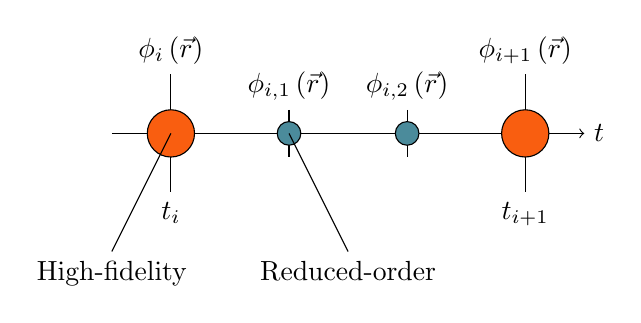
\begin{tikzpicture}[scale=3]
        \draw[->] (-0.25,0) -- (1.75, 0) node[anchor=west] {$t$};
        \draw (0,0.25) node[anchor=south] {$\phi_i\left(\vec{r}\right)$} --
            (0,-0.25) node[anchor=north] {$t_{i}$};
        \draw (1.5,0.25) node[anchor=south] {$\phi_{i+1}\left(\vec{r}\right)$} --
            (1.5,-0.25) node[anchor=north] {$t_{i+1}$};
        \filldraw[fill=tikzbetterred] (0,0) circle (0.1);
        \filldraw[fill=tikzbetterred] (1.5,0) circle (0.1);
        \foreach \y in {0.5,1} {
            \draw (0+\y,0.1) -- (0+\y,-0.1);
            \filldraw[fill=tikzbetterblue] (0+\y,0) circle (0.05);
        }
        \draw (0.5, 0.1) node[anchor=south] {$\phi_{i,1}\left(\vec{r}\right)$};
        \draw (1, 0.1) node[anchor=south] {$\phi_{i,2}\left(\vec{r}\right)$};
        \draw (-0.25, -0.5) node[anchor=north] {High-fidelity} -- (0, 0);
        \draw (0.75, -0.5) node[anchor=north] {Reduced-order} -- (0.5, 0);
    \end{tikzpicture}
    \caption{Depiction of a mixed-fidelity substep depletion scheme}
    \label{fig-substep_flow}
\end{figure}

Between substeps, it is useful to extrapolate microscopic reaction cross sections.
This allows the reaction rates used to deplete at the substeps to better reflect
the ``true'' reaction rates.
Furthermore, one may need to construct macroscopic cross sections for the reduced-order
solver in order to obtain the substep fluxes.
To this end, microscopic cross sections are computed by the high-fidelity code
and stored for extrapolation.

A Python package was developed in order to implement and test the hybrid coupling
scheme, as no such tool exists in the field.
When developing this framework, emphasis was placed on abstraction and extensibility.
By carefully abstracting away functionality from monolithic blocks into classes with
succinct purposes and interfaces, the framework can easily be extended in the future.
The full framework can be obtained as an open-source package\footnote{%
    \url{https://github.com/CORE-GATECH-GROUP/hydep}}.

The key aspects of the framework are two abstract interfaces for generic
high-fidelity and reduced-order transport codes.
These interfaces perform no computational benefits, instead serving
as base classes for useful interfaces.
With this approach, it would be much easier to incorporate additional transport
solvers without having to rework the entire computational sequence.
Developers need not worry about storing reaction cross sections or even exporting
result data to disk, as these are handled by other classes in the framework.
Instead, transport interfaces must be able to
\begin{enumerate}
    \item{initialize a solver-specific representation of the materials and geometry;}
    \item{update material information given post-depletion burnable material definitions;}
    \item{execute a transport solution; and}
    \item{return back to the framework results including, at a minimum, scalar fluxes.}
\end{enumerate}

Reduced-order solvers and the depletion backend communicate what physics are necessary
to the high-fidelity solver, which in turn should be aware of what physics are supported
(e.g., spatial homogenization to obtain few-group macroscopic cross sections, fission matrix,
collapsing of microscopic cross sections).
This allows the framework to ensure compatibility between solvers that may have been developed independently.
In the event the high-fidelity solver does not support some of the physics required,
the framework safely terminates before any expensive work has been completed.

The Serpent interface is responsible for building the initial model of the problem,
including geometry and necessary tallies, executing Serpent, and processing
the coarse step results.
The serpentTools Python package \cite{Johnson2020SerpenttoolsPythonPackage} is used
to obtain fluxes, multiplication factor, homogenized macroscopic cross sections,
and other required data.

A modified Serpent version was developed that allows the user to update compositions
through text files while cross section data and model representation are retained in memory.
This modification means that, at the beginning of each coarse step, Serpent does not
have to restart fully from scratch.
Instead, Serpent reads this data file, updates compositions of burnable materials,
and then proceeds into the transport solution.
While the distribution of this patched version is underway, an interface for the distributed
Serpent 2.1.31 also exists in the framework.

The reduced-order solution initially chosen for this work is the spatial flux variation
method (SFV) introduced in~\cite{Johnson2020TransportFreeMethod}.
It uses first-order perturbation theory to predict the change in scalar neutron
flux between two state-points, identified with macroscopic neutron absorption and
fission neutron production cross section.
The beginning-of-step (BOS) fission matrix and multiplication factor are also
necessary to perform the prediction.
An interface into a small Python-wrapped Fortran library\footnote{\url{https://github.com/CORE-GATECH-GROUP/sfv}}
was developed to predict, normalize, and return the substep fluxes.

Using the current compositions and reaction rates across all materials,
the package uses the incomplete partial factorization (IPF) formulation
of CRAM to update compositions~\cite{Pusa2016HigherOrderChebyshev,Pusa2010ComputingMatrixExponential}.
The implementation and some data structures are inspired by the OpenMC depletion module%
~\cite{Romano2020DepletionCapabilitiesOpenmc}, and heavily relies on the NumPy
and SciPy Python packages~\cite{Walt2007NumpyArrayStructure,Jones2001ScipyOpenSource}.
This implementation has been verified against the Serpent internal depletion solver
in previous work by the authors~\cite{Johnson2020TransportFreeMethod}.

\section{TEST PROBLEM}

The hybrid depletion method was compared to a 3-D PWR pincell model spanning 360\ cm.
This model is similar to test problems used in
\cite{Densmore2013StabilityAnalysisBurnup,Johnson2020TransportFreeMethod}
and other depletion studies with a focus on numerical stability.
With initially symmetric compositions and axially vacuum boundary conditions, one
would expect the flux and power profiles to begin as a symmetric waveform
with a global maximum at the midpoint.
However, as has been found in the aforementioned papers, there is a depletion step size
that, if exceeded, can lead to asymmetric and oscillatory solutions.

A reference solution was generated using the Serpent predictor-corrector with
single day depletion steps.
A reflective boundary condition was place at the axial mid-point in order to remove
instabilities from the reference model.
Detailed isotopic comparisons will not be presented between the hybrid scheme and the
Serpent reference as the different depletion implementations would obfuscate the impact,
positive or negative, of the hybrid depletion scheme.
More detailed comparisons will be the subject of a future publication.

The Serpent predictor and hybrid depletion scheme both used five and ten day depletion
steps following ten single-day steps.
This initial period allowed for some fission product inventory to be built up and more
reliable microscopic reaction cross sections to be stored.
Due to spectral changes and a step change in number densities of fission products,
extrapolation of these cross sections from day zero with fresh fuel is not ideal:
the large change in one-group cross sections across this first step is likely
sharper than subsequent points and should not be used in the extrapolation.

All models were depleted out to day 310 using a power density of 0.04 kW/g HM.
In all cases, the entire 360\ cm fuel pin was subdivided into 100 equal-volume
axial layers.
In each section, the one-group neutron scalar flux was tallied, and atom densities
of relevant nuclides were reported.
The scalar flux was used to compute the axial offset using
\begin{equation} \label{eq-ao}
    AO \equiv \frac{
        \sum_{l=N/2+1}^N\phi_l
    }{
        \sum_{l=1}^{N}\phi_l
    } - 0.5
\end{equation}
where a positive value indicates more scalar flux in the top half of the pin
and a perfectly symmetric solution has an axial offset of zero.
Multiplication factors will be compared using
\begin{equation} \label{eq-dk}
    \Delta k\ [pcm] \equiv \frac{k^\prime - k_{ref}}{k_{ref}} \times 10^5.
\end{equation}

The hybrid results were generated using single-day substeps inside the five and
ten day coarse steps.
Three-point linear extrapolation of microscopic cross sections was found to work
well for a similar problem in~\cite{Johnson2020TransportFreeMethod} and
was used in this work.
The substep flux at day 12, for example, was computed with
    the SFV method using compositions from day 12,
    multiplication factor and fission matrix from the previous high-fidelity solution at day ten, and
    macroscopic reaction cross sections extrapolated from days eight, nine, and ten.

\section{RESULTS}

\cref{fig-ao} presents the axial offsets, computed by \cref{eq-ao} for the hybrid
depletion scheme and the Serpent predictor.
For context, the axial scalar flux shapes for each case are presented in \cref{fig-fluxes}.
The maximum uncertainty on the day zero bin-wise scalar flux was less than one percent.
Results like those presented for the predictor have been reported in the literature,
but it still serves as a point of comparison for the hybrid depletion scheme presented here:
both are explicit schemes using only the beginning-of-step reaction rates to deplete across
a time step.

\begin{figure}
    \includegraphics{axial_offsets.pdf}
    \caption{Axial offsets for the hybrid depletion sequence compared to the predictor scheme}
    \label{fig-ao}
\end{figure}

\begin{figure}
    \includegraphics{fluxes.pdf}
    \caption{Scalar flux shapes for fuel pin. Top row contains result with five
    day depletion steps after day ten. Bottom row uses ten day steps}
    \label{fig-fluxes}
\end{figure}

This improved stability lends itself to a more accurate estimation on $k$, as evidenced
in~\cref{fig-dk}.
Uncertainty was not propagated through the depletion calculation, but the maximum single-step
uncertainty on $k$ was 12 pcm across all cases.
\cref{fig-dk} indicates that the multiplication factor produced by the hybrid scheme is
at or near two standard deviations away from the Serpent reference for the entire
310 day irradiation period.
Furthermore, there is little difference in the values produced using five or ten day
coarse steps for the hybrid scheme.
Comparatively, both the five and ten day predictor cases result in 1700-2000 pcm
of difference.

\begin{figure}
    \includegraphics{hybrid_ce_dk.pdf}
    \caption{Difference against reference multiplication factor for hybrid scheme (left)
    and Serpent predictor-corrector reference (right).}
    \label{fig-dk}
\end{figure}

Including the calculation of the fission matrix, necessary for the SFV prediction, into
the hybrid solution increased the simulation time by 8.7\%.
The SFV prediction requires orders of magnitude less time than the high-fidelity Monte
Carlo solution and has negligible impact on overall simulation time.
By comparison, just halving the step size from five to 2.5 days increases the number of
transport simulations from 70 to 130, provided both cases use ten initial single day steps.
Assuming each transport simulation requires roughly the same simulation time, this translates
to an 85\% increase in simulation time.

\section{CONCLUSIONS}

The use of smaller depletion steps has been shown to improve the stability
and accuracy of a coupled transport-depletion simulation, especially for
problem with a high dominance ratio
\cite{Kotlyar2013UsePredictorCorrector,Densmore2013StabilityAnalysisBurnup}.
Decreasing the depletion step, however, requires more potentially expensive transport
simulations.
This work presented a hybrid depletion scheme where reduced-order simulations
are coupled between high-fidelity solutions in a substep manner.
The use of substeps allows smaller depletion steps to be used but the computational burden
is shifted onto the reduced-order simulations.

As shown in this work, the solution obtained by this hybrid scheme does not experience
the well-reported oscillations and instabilities for this stability-limited problem.
The global multiplication factor was within 35 pcm of the reference predictor-corrector
solution.
As the reference solution was computed using a single day predictor-corrector, involving
two transport solutions per step, the five and ten day hybrid solutions used 89\% and 93\%
fewer transport simulations, respectively.

\section*{ACKNOWLEDGMENTS}
This work was partially funded through U.S. Regulatory Commission project number
HQ-84-14-G-0058.
The patched Serpent version was developed with inspiration and guidance from Jaakko Lepp\"anen
and Ville Valtavirta.
Relevant data files and processing scripts for this work can be found at
\url{https://github.com/CORE-GATECH-GROUP/mc21-depletion}.

\setlength{\baselineskip}{12pt}
\bibliographystyle{mc2021}
\bibliography{references/references.bib}

\end{document}
